\chapter{NOOSFERO}

O Noosfero é uma plataforma \textit{open source} para a construção de redes sociais
e colaborativas. Desenvolvido em Ruby on Rails e licenciado sob AGPL versão 3, o
projeto ainda conta com desenvolvimento ativo.

Além dos mecanismos de interação social, o Noosfero também conta com um sistema de
gerenciamento de conteúdo, o que possibilita a criação de \textit{blogs} e o
compartilhamento de arquivos. A plataforma também pode ser estendida por
\textit{plugins} desenvolvidos pela comunidade, e conta com o conceito de
\textit{environments}, que permitem a criação de diversas redes isoladas funcionando
sobre uma mesma instância da aplicação.

\begin{figure}[h]
	\centering
		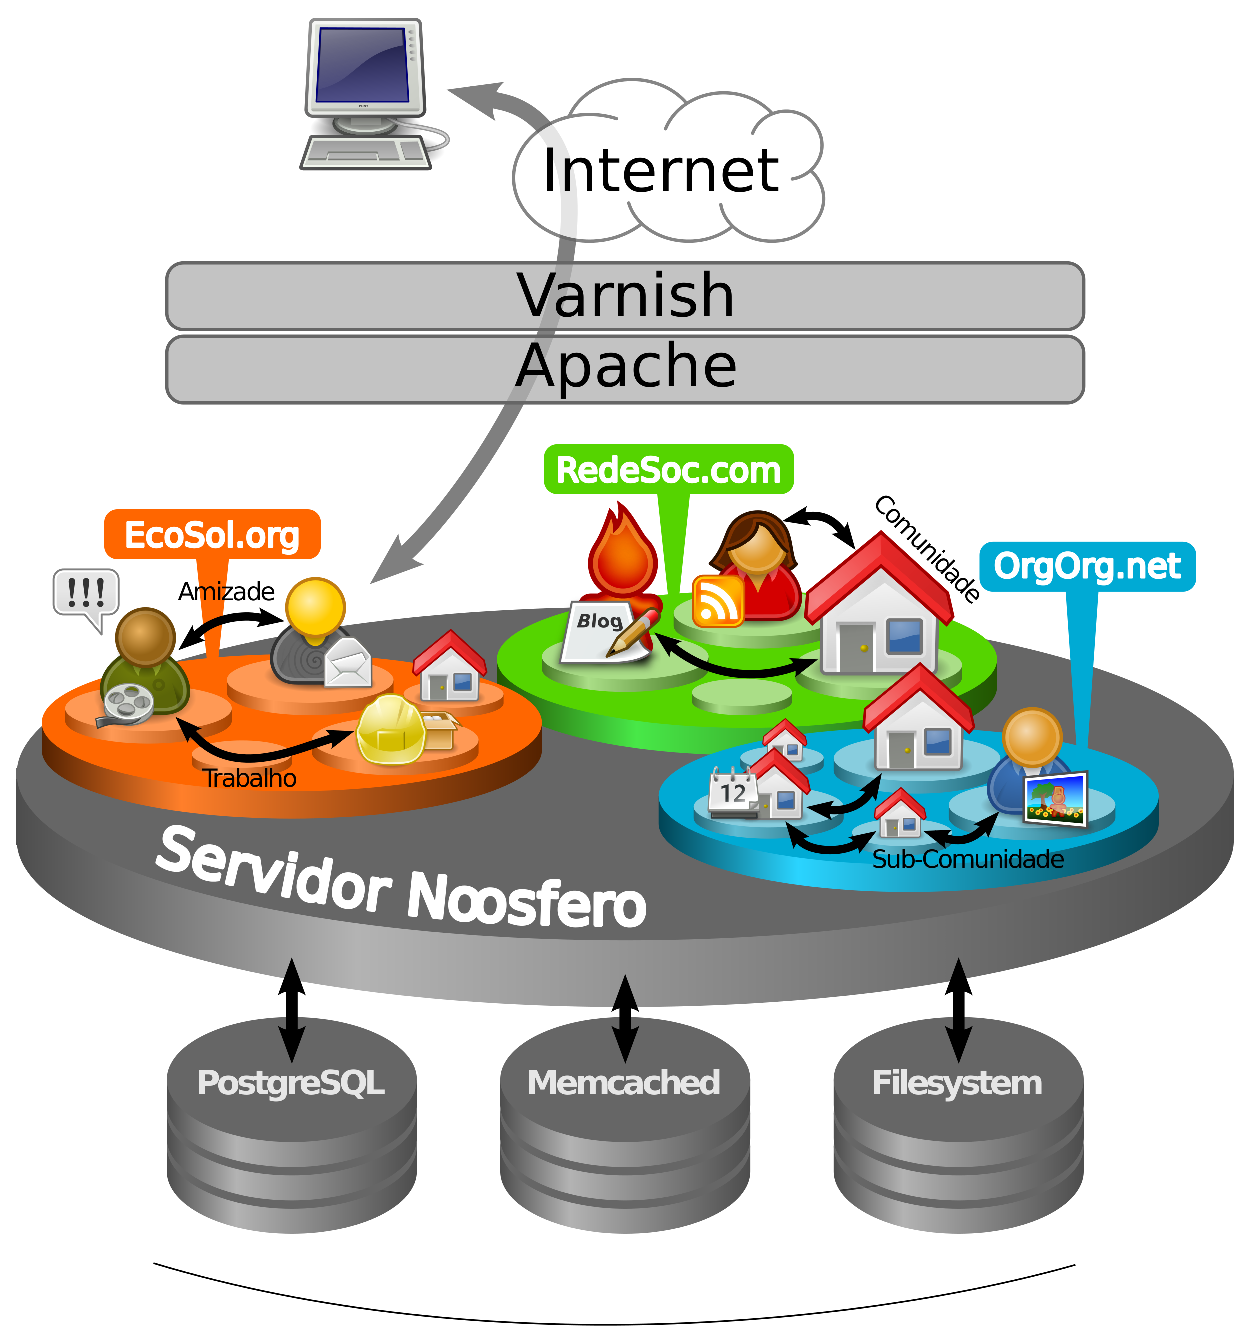
\includegraphics[keepaspectratio=true,scale=0.4]{figuras/noosfero_estrutura.eps}
	\caption{Arquitetura do Noosfero}
	\label{fig:noosferoEstrutura}
\end{figure}
% adicionar fonte

As informações e publicações de pessoas e organizações podem ser públicas ou
privadas. Já os relacionamentos entre estas entidades podem ser tanto simétricos
como assimétricos.

Enquanto um relacionamento simétrico depende da concordância de ambas as partes para
o compartilhamento das informações privadas (como por exemplo amizades ou
filiações), um relacionamento assimétrico depende apenas do interesse de uma das
entidades em acompanhar as informações públicas de algum perfil (como no caso da
funcionalidade de seguidores).



\section{SUPORTE À FEDERAÇÃO}

As definições da federação no Noosfero surgiram no contexto de desenvolvimento do
projeto do Portal do Software Público, como resultado de uma consultoria executada
pela Cooperativa de Tecnologias Livres \cite{colivre2016}. O produto foi um
relatório que define os objetivos e requisitos da implementação de federação na
plataforma Noosfero.

A proposta é que seja possível realizar a integração não só com outras instâncias do
Noosfero, como também com outras redes sociais. Desta forma, é necessário adotar
especificações que tenham o mínimo de aderência na comunidade, ao menos em outros
projetos que investem na implementação da federação entre redes sociais. Os
protocolos Diaspora e OStatus foram escolhidos observando projetos como o Hubzilla,
Friendica, e o próprio Diaspora.

É interessante que mesmo a integração entre redes Noosfero respeite os padrões
adotados pelos protocolos de referência, evitando a criação de outro padrão que não
reconhecido pelo restante dos projetos. No entanto, implementar a federação
respeitando os padrões existentes pode exigir uma refatoração da arquitetura ou das
funcionalidades da plataforma. Por exemplo, nenhum dos protocolos de referência
respeita o conceito de relacionamentos simétricos, padrão no Noosfero até então.


\subsection{Federação entre redes Noosfero}

As primeiras contribuições com a federação no Noosfero foram na integração de
instâncias diferentes da plataforma. As atividades foram definidas de acordo com
um \textit{roadmap} que dividiu a implementação em quatro fases, que cobrem desde
a reestruturação da arquitetura da aplicação, até a construção dos mecanismos
necessários para a autenticação e relação entre as redes.

% TODO: que funcionalidades devem ser oferecidas para um usuário federado

O protocolo construído entre redes Noosfero é baseado nas especificações do
WebFinger e OAuth para a descoberta de identidade e autorização de perfis,
respectivamente. Em relação à comunicação entre as redes, o protocolo Diaspora foi
definido como referência. 

\subsubsection{Fase 1: preparação}

Até a versão 1.5 do Noosfero, todos os relacionamentos entre as entidades da rede
eram baseados no conceito de relacionamento simétrico. No entanto, a aderência

Na fase de preparação foram introduzidos os relacionamentos assimétricos através da
funcionalidade de seguidores. Seguidores podem visualizar as atividades e
informações públicas

\subsubsection{Fase 2: intercomunicações}

% WebFinger, ExternalX...
% Autenticação, comentários...
% Sugestão de artigos?

\subsubsection{Fase 3: integração externa}

% Evolução do oauth

\subsubsection{Fase 4: inter-relações}

% Relações entre usuários de diferentes redes


\subsection{Federação com outras redes sociais}

A implementação da federação com redes não Noosfero devem usar a infraestrutura
desenvolvida para a integração entre redes Noosfero, principalmente os mecanismos
de usuários externos e troca de mensagens.

% TODO: essas aplicações foram escolhidas com base em que?
Já que não existe um padrão para a federação de redes sociais, inicialmente é
necessário oferecer suporte a aplicações individuais. Dedicou-se atenção especial
aos projetos que contam com iniciativas de federação significativas, precisamente
os projetos Diaspora, Hubzilla, Friendica, e GNU Social.

% TODO: adicionar referência para o suporte que os projetos oferecem (nota de rodapé)
Com exceção do GNU Social, os projetos que serão inicialmente suportados atendem às
especificações do protocolo Diaspora. O suporte às redes baseadas no OStatus será
oferecido implementando uma parte dos protocolos desta suíte, como o Salmon, o
Activity Streams e o PubHubSub.

Para que a federação seja bem sucedida, é essencial garantir que a integração seja
bidirecional. Além de permitir que usuários acessem e interajam com uma rede
Noosfero com o perfil de outra rede social, um usuário Noosfero também devem
conseguir fazer o mesmo em qualquer uma destas redes. Além da autorização, a
federação depende da descentralização dos conteúdos, o que exige que as interações
possam acontecer em qualquer uma das redes, mas que o estado seja sempre o mesmo
em cada uma delas.

De modo geral, as mesmas funcionalidades implementadas na federação de redes
Noosfero deve ser suportada, desde que toda interação exerça impacto tanto na rede
de origem quanto na rede federada, sejam estas instâncias Noosfero ou não.

As atividades necessárias para a implementação desta etapa de federação podem ser
organizadas nas etapas descritas a seguir.

% TODO: o que o Diaspora suporta e não suporta?
% TODO: o que especificamente deve ser implementado no OStatus?

\begin{enumerate}
  \item{Possibilitar o gerenciamento das redes federadas através de um  mecanismo de 
        \textit{whitelist} para a autorização de redes não Noosfero, o que deve
        incluir a avaliação de um mecanismo de descoberta para as redes existentes;}

  \item{Possibilitar um usuário possa acessar outras redes com as credenciais de sua
        rede de origem, sem a necessidade de um novo cadastro;}
        % Evolução do plugin de OAuth ou utilização do WebFinger?

  \item{Permitir relações assimétricas entre usuários de redes distintas através do
        protocolo Diaspora. Permitir que as atividades (\textit{feed}) sejam
        visualizadas tanto na redes de origem quanto na federada;}

  \item{Possibilitar interações a partir de qualquer uma das redes através do
        protocolo Diaspora, o que evita que, por exemplo, um usuário precise acessar
        outro domínio para comentar uma publicação. Os usuários envolvidos na
        interação devem ser notificados em suas redes de origem.}

  \item{Permitir relações assimétricas e interações através dos protocolos indicados
        na especificação do OStatus, com os mesmos fins da implementação através do
        Diaspora;}
\end{enumerate}

% TODO: (no caso do Diaspora: o que inclui tais e tais funcionalidades...)
No desenvolvimento deste trabalho será priorizado a implementação da federação
através do protocolo Diaspora. Indica-se a expansão da federação por meio do OStatus
como um trabalho futuro.

\subsubsection{Implementação do Protocolo Diaspora}



